\documentclass[a4paper,12pt]{article}
\usepackage{natbib}

\usepackage[brazil, english]{babel}
\usepackage[latin1]{inputenc}
\usepackage[T1]{fontenc}
\usepackage{color}
\usepackage{ulem} 

\usepackage{amsmath}
\usepackage{lineno}

\usepackage{graphicx}
\graphicspath{{../../text/figuras/}}
\usepackage{epsfig}


\usepackage{multirow}

\usepackage{array}
\newcolumntype{M}[1]{>{\centering\arraybackslash}m{#1}}
\newcolumntype{N}{@{}m{0pt}@{}}

\usepackage{hyphenat}

\bibliographystyle{amsplnat}


\title{Nonlinear modeling of the gasoline/ethanol share on ozone concentration}
\author{William Nilson Amorim, Antonio Carlos Pedroso de Lima, \\ Julio M. Singer,  Carmen D.S. Andr�, \\
{\small Departamento de Estat�stica, Universidade de S�o Paulo, Brazil} \\
Maria de F�tima Andrade, \\
{\small Departamento de Ci�ncias Atmosf�ricas, Universidade de S�o Paulo, Brazil} \\
Paulo H.N. Saldiva \\
{\small Instituto de Estudos Avan�ados, Universidade de S�o Paulo, Brazil}
}
\date{}

\begin{document}
	
%\linenumbers
	
\maketitle

Bio-ethanol, a quasi-renewable fuel widely used in some countries as a cleaner option than gasoline, has been in the focus of the energy agenda since the European Commission stated that by 2050 the European Union should cut 20\% of the greenhouse gas emissions relatively to 1990 levels and increase to 20\% the amount of renewable energy used.

The ethanol/gasoline shift as vehicles fuel is directly associated with the atmospheric balance of nitrate oxides (NOx) and organic volatile composts (VOCs), since gasoline burning generates more NOx and ethanol evaporation and partial burning generates more VOCs. This balance is an important component to describe the tropospheric ozone formation along the day \cite{SashaMadronich2014}. 

In the past years, some have discussed the actual impact of shifting gasoline to ethanol as primary fuel in bi-fuel light-duty vehicles. \cite{Salvo2014} showed that ozone concentration decreased as the share of bi-fuel vehicles burning gasoline rose from 14 to 76$\%$ in S�o Paulo, Brazil, analyzing data from 2008 to 2011, and shed a valid concern about whether ethanol is a safer substitute for gasoline with respect to its relation with ozone concentration.

Besides ozone, particulate matter has also been subject of many air pollution studies, mostly for the lack of regulation, lack of a safe threshold, and its effects on public health. \cite{Salvo2017} extended this work analyzing data from 2008 to 2013 and other pollutants, like fine particles. The authors reached the same conclusion for ozone concentration, but they observed that ambient number concentrations of 7?100nm diameter particles (ultra-fine particles) rise along with the use of gasoline.

This work has as primary goals (1)  analyze if the association between ozone and the estimated proportion of vehicles burning gasoline is in fact linear and (2) investigate the association between mortality and the estimated proportion of vehicles burning gasoline. To reach this goals, we used more sophisticated non-linear models, such as generalized addictive models and random forests, as well the LIME method to interpret the results of the latter.


\section{Pollution, weather and traffic data}

The data used in this study was collected, organized and provide by \cite{Salvo2017}. It consist of air pollution, meteorologic and traffic data, as well the \textit{shareE25}, the estimated proportion of bi-fuel vehicles burning gasoline with 25\% ethanol (E25) over pure ethanol (E100).

The \textit{shareE25} variable was estimated using information on the price of ethanol at the pump and the motorist-level revealed-choice survey data \citep{Salvo2013}. Such values were estimated weekly for the entire city, implying that the proportion of bi-fuel vehicles running on E25 was the same for all the monitoring stations where the pollutants were recorded hourly.

The air pollution and meteorologic data was measured hourly in several monitoring stations along the city  maintained by the environmental authority of the state of S�o Paulo (CETESB). The traffic data, also measured hourly, was provided by the city traffic authority (CET).

More information about the data can be found in supplementary information of \cite{Salvo2014} and \cite{Salvo2017}.

\section{Statistical analysis}

To analyze the effect of the \textit{shareE25} variation on the ozone levels, \cite{Salvo2017} used a linear regression model, which assumes that the relation between this to variables is the same for all the values of \textit{shareE25}.

To investigate the linearity assumption, we applied two non-linear models on the exactly same variables considered by the authors. The first is the well established \textit{generalized additive model} \citep{Hastie2008}, which allows one to associate each one of the predictors to the response variable using a non-linear function. The second one is a \textit{bagging} tree model known as \textit{random forest}. This model consider a high number of regression trees and average its results to make predictions. Due to the lack of interpretation,  this type of predictive model is very little used in studies where the main goal is to make associations between variables. To work around this problem, we used a interpretation technique called LIME \citep{Ribeiro2016}.

More details about this models can be found in \cite{James2013}.

Following \cite{Salvo2017}, we used as response the daily 12pm to 7pm ozone concentration average, excluding the cold months from June to September. We have ozone data available from 12 monitoring stations in the city. We also considered the same predictors as the authors presented in the Table \ref{tab:variaveis-modelo-salvo-2017}.

\begin{table}[h!]
	\centering
	\caption{Predictors considered for the ozone models}
	\begin{tabular}{M{2cm}|M{8cm}|M{3cm} N}
		\hline 
		Type & Variables & Number of parameters & \\[10pt]
		\hline 
		Ethanol & Estimated proportion of cars running by gasoline (E25) & 1 & \\[10pt]
		\hline
		Station & Monitoring station dummies. & 11 & \\[10pt] 
		\hline
		Calendar & Dummies for day of week, week of year, vacation periods and public holidays.  &  44 & \\[10pt] 
		\hline 
		Trend & General and station specific trend term. &  12 & \\[10pt] 
		\hline 
		Climate & Temperature, solar radiation, humidity, wind speed and dummies for precipitation and thermal inversion.. & 9 & \\[10pt]
		\hline 
		Traffic & Dummies for station specific and city vehicle traffic intensity, as well inauguration of important beltway. & 18  & \\[10pt]
		\hline 
		\textbf{Total} & \textbf{16 predictors + intercept term} & \textbf{96 parameters*}  & \\[10pt]
		\hline
	\end{tabular}
	\\
	\vspace{1mm}
	\scriptsize{*95 parameters from predictors + 1 parameters from intercept term.}
	\label{tab:variaveis-modelo-salvo-2017}
\end{table}

The model considered by \cite{Salvo2017} estimated a coefficient of -16.66 $\pm$ 10.01 to the \textit{shareE25} variable, suggesting that the increase of the proportion of cars burnning E25 in the city is associated with the decrease of ozone levels. To compare the models, we used the root mean square error estimated by cross validation. We also compute the proportion of variance explained for each model. For the model used by \cite{Salvo2017}, these two quantities were, respectively, 19.74 and 70.65\%.

\section{Results}

We fitted three generalized additive models, the first using the Normal distribution, the second using the Gamma distribution and the last using the Inverse Normal distribution. The non-linear functions were assign to all numeric predictors: \textit{shareE25}, temperature, radiation, humidity, wind speed and trend. The other predictors were linear associated with the response. Smoothing splines were used to estimate the functions and the smoothing degree was chosen by cross validation. In the three models, the \textit{shareE25} variable was considered statistically significant to explain the ozone concentration. The performance of each model is described in the Table \ref{tab:cap-comb-resultados-gam}.

\begin{table}[h!]
	\centering
	\caption{Resultado dos modelos aditivos generalizados utilizados para ajustar os dados de \cite{Salvo2017}.}
	\begin{tabular}{M{2cm}|M{1cm}|M{2cm}|M{6cm} N}
		\hline
		Distribui��o & RMSE & \% var. explicada & Vari�veis mais importantes &\\
		\hline
		Normal & 19.82 & 70.50 & Temperatura, vento, umidade, radia��o e tend�ncia &\\
		Gama & 20.07 & 69.50 & Temperatura, vento, umidade, radia��o e tend�ncia  &\\
		Normal inversa & 29.28 & 45.30 & Temperatura, radia��o, umidade, vento e tend�ncia &\\
		\hline
	\end{tabular}
	\label{tab:cap-comb-resultados-gam}
\end{table}

The results from the Normal and Gama models were close to those for the linear regression fitted by \cite{Salvo2017}, while the Inverse Normal model got bigger RMSE and lower R$^2$, indicating that this distribution is not appropriated to fit the data. Contrary to the linear regression model, the trend term was held as one of the five most important variables to explain the variability of the ozone concentration in these three models. It presumably happened due to the flexibility of the GAM to represent the non-linearity of this temporal component. The \textit{shareE25} variable was the 13th more important in the Normal model, and the 9th in the Gama model and Inverse Normal model.

The usual method to interpret the generalized additive models is to plot each predictor by its estimated non-linear function. Figure \ref{fig:comb-gam-plot} shows this plot for the \textit{shareE25} variable, suggesting a non-linear relation between this variable and the concentration of ozone: positive in the extremes (10\% - 20\% and 60\% - 80\%) and negative in the center (20\% - 60\%).

\begin{figure}[h!]
	\centering
	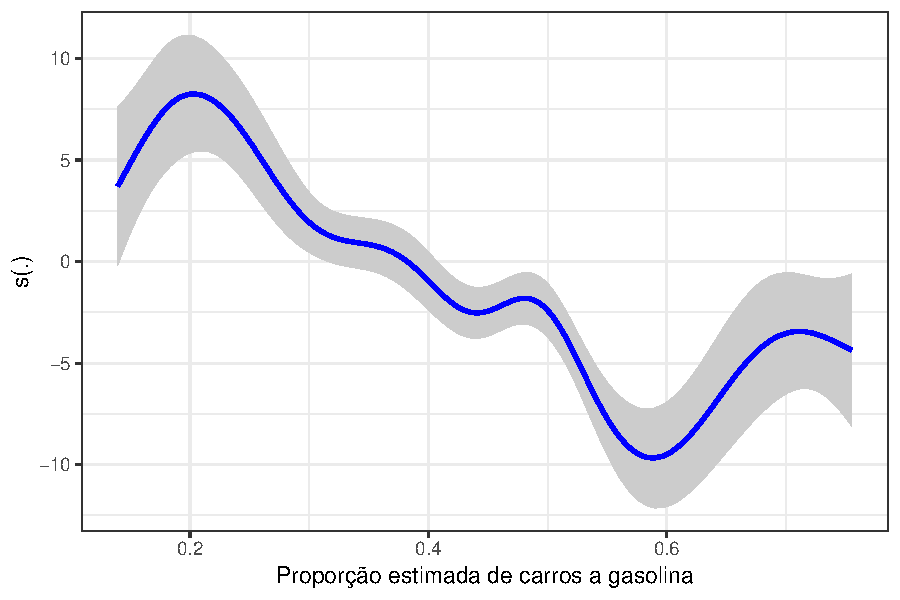
\includegraphics[width=0.7\linewidth]{cap-comb-gam-plot.pdf}
	\caption{Non-linear function estimated by the Normal generalized additive model to the \textit{shareE25} variable. The gray area represents a 95\% confidence interval.}
	\label{fig:comb-gam-plot}
\end{figure}

To evaluate the variability of the estimates, we also followed the strategy in \cite{Salvo2017} and fitted the Normal GAM (which had the best performance) in 200 bootstrap samples. Figure \ref{fig:comb-gam-plot-bs} shows the 200 estimated curves (in gray) for the \textit{shareE25} variable in the bootstrap models and the cubic splines smoothed curve (in blue). The non-linear pattern found is the same as described earlier. The high variability in the extremes is result of few data with low or high estimated proportion of cars burning E25.


\begin{figure}[h!]
	\centering
	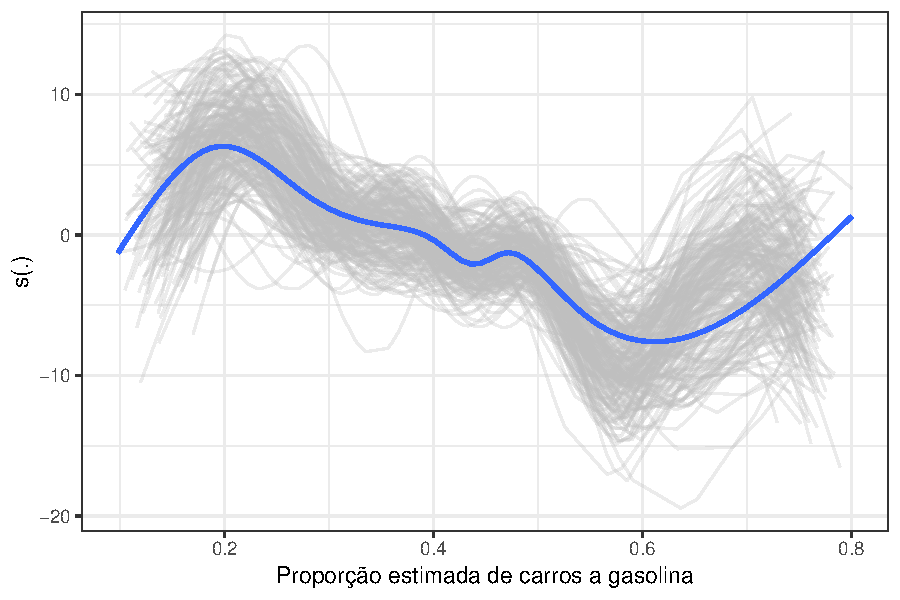
\includegraphics[width=0.7\linewidth]{cap-comb-gam-plot-bs.pdf}
	\caption{In gray, the 200 estimated curves for the \textit{shareE25} variable in the bootstrap models. In blue, the cubic splines smoothed curve.}
	\label{fig:comb-gam-plot-bs}
\end{figure}

The table \ref{tab:cap-comb-resultados-random-forest} shows the results of the random forest model. As expected we obtained a lower test error (RMSE = 14.11) and higher R$^2$ (85.72) than the linear regression and the additive models. The five most important predictors were: temperature, humidity, radiation, wind speed e trend, just like in the GAM. The \textit{shareE25} was the 6th most important variable. 

\begin{table}[h!]
	\centering
	\caption{Random forest model results for the \cite{Salvo2017} data. The hyperparameters for minimal node size and number of predictors sampled in each tree were chosen by cross validation.}
	\begin{tabular}{M{2cm}|M{3cm}|M{2cm}|M{2cm}|M{5cm} N}
		\hline
		Minimal node size  & Number of predictors sample & RMSE & \% var. explained & Most important variables & \\
		\hline
		1 & 48  & 14.11 & 85.72 & Temperature, humidity, radiation, wind speed e trend & \\
		\hline
	\end{tabular}
	\label{tab:cap-comb-resultados-random-forest}
\end{table}

Although we have a more precise fit, we can not directly access  the relation between the \textit{shareE25} and the ozone concentration, i.e., we don't know if this predictor is statistically significant to explain the variability of the ozone levels and the direction of this supposed association. To solve this problem, we used the LIME technique to interpret the results of the random forest. With this goal in mind, we chose to evaluate the \textit{shareE25} effect on the 100 days with the lower levels of ozone and the 100 days with the higher levels. Figure \ref{fig:cap-comb-lime-pinheiros} suggests that, for the days with high ozone concentration, the protective effect of the \textit{shareE25} happens mostly when more then 50\% of the fleet is burning gasoline. The same happens on the days with lower ozone concentration. This pattern support the hypothesis of non-linear relation between these ozone concentration and ethanol/gasoline burning.

\begin{figure}[h!]
	\centering
	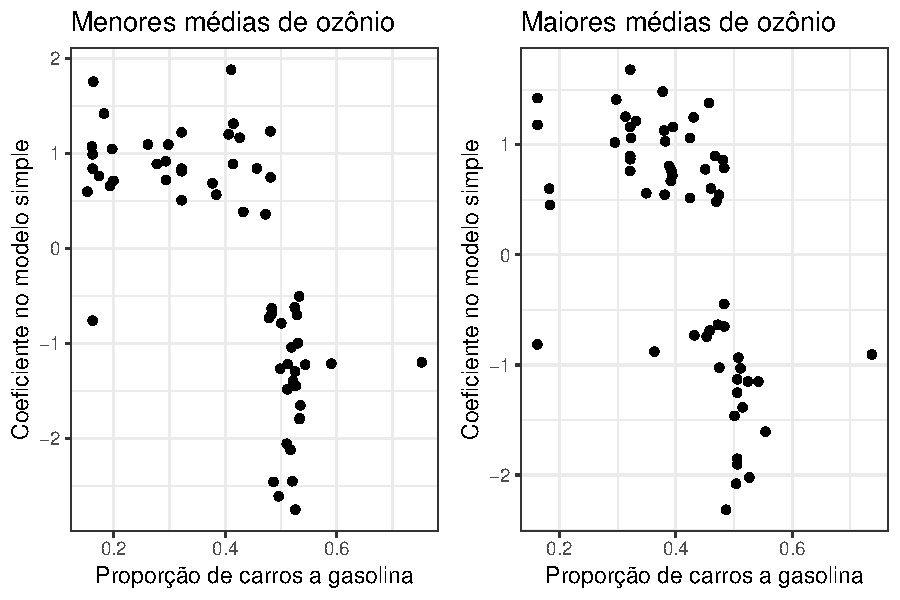
\includegraphics[width=0.7\linewidth]{cap-comb-lime-pinheiros.pdf}
	\caption{\textit{shareE25} against the estimated coefficient for this predictor in the simple model used in LIME (ridge regression). On the left, the 100 days with lower ozone concentration. On the right, the 100 days with higher ozone concentration.}
	\label{fig:cap-comb-lime-pinheiros}
\end{figure}



\section{Discussion}

%\newpage
%\bibliography{C:/Users/William/Dropbox/Latex/Bibs/atlas.bib}
%\bibliography{/home/acarlos/Dropbox/FAPESP/Tematicos/MODAU/Ozonio/atlas.bib}
%\bibliography{/home/jmsinger/Dropbox/MODAU/Etanol/atlas.bib}
\bibliography{../../../Latex/Bibs/atlas.bib}
			
\section*{Acknowledgements} 

This research received financial support from Coordena��o de Aperfei�oamento de Pessoal de N�vel Superior (Capes), Conselho Nacional de Desenvolvimento Cient�fico e Tecnol�gico (CNPq, grant 3304126/2015-2)
and Funda��o de Amparo � Pesquisa do Estado de S�o Paulo (FAPESP, grant 2013/21728-2), Brazil.
 			
\section*{Author contributions}

W.N.A., A.C.P.L., J.M.S. and C.D.S.A. analyzed the data; M.F.A. contributed with climate and pollutant chemistry knowledge; P.H.N.S. suggested the theme; all authors wrote the paper.

\section*{Additional information}

Correspondence and request for materials should be addressed to W.N.A.
All the figures and the R codes used in the statistical analysis may be obtained respectively at  http://bit.do/amorim\_et\_al\_figures and \\ http://bit.do/amorim\_et\_al\_codes. 

\section*{Competing financial interests}

The authors declare no competing financial interests.


\end{document} 

